\newpage
\section{ヘッドセットの使い方}
\ruby{演習}{えん|しゅう}の前に、ヘッドセットの\ruby{設定}{せっ|てい}をしましょう。ヘッドセットとは、コンピュータなどから音声を出力するためのヘッドフォンと、コンピュータなどに音声を入力するためのマイクが一体型になったものです。\\
まずはラズベリーパイの\ruby{電源}{でん|げん}を入れる前に、ヘッドセットとラズベリーパイをつないでおきます。
ヘッドセットがラズベリーパイに\ruby{接続}{せつ|ぞく}されていると、画面の右上にマイクのアイコンが追加されます。

\begin{figure}[H]
\begin{center}
    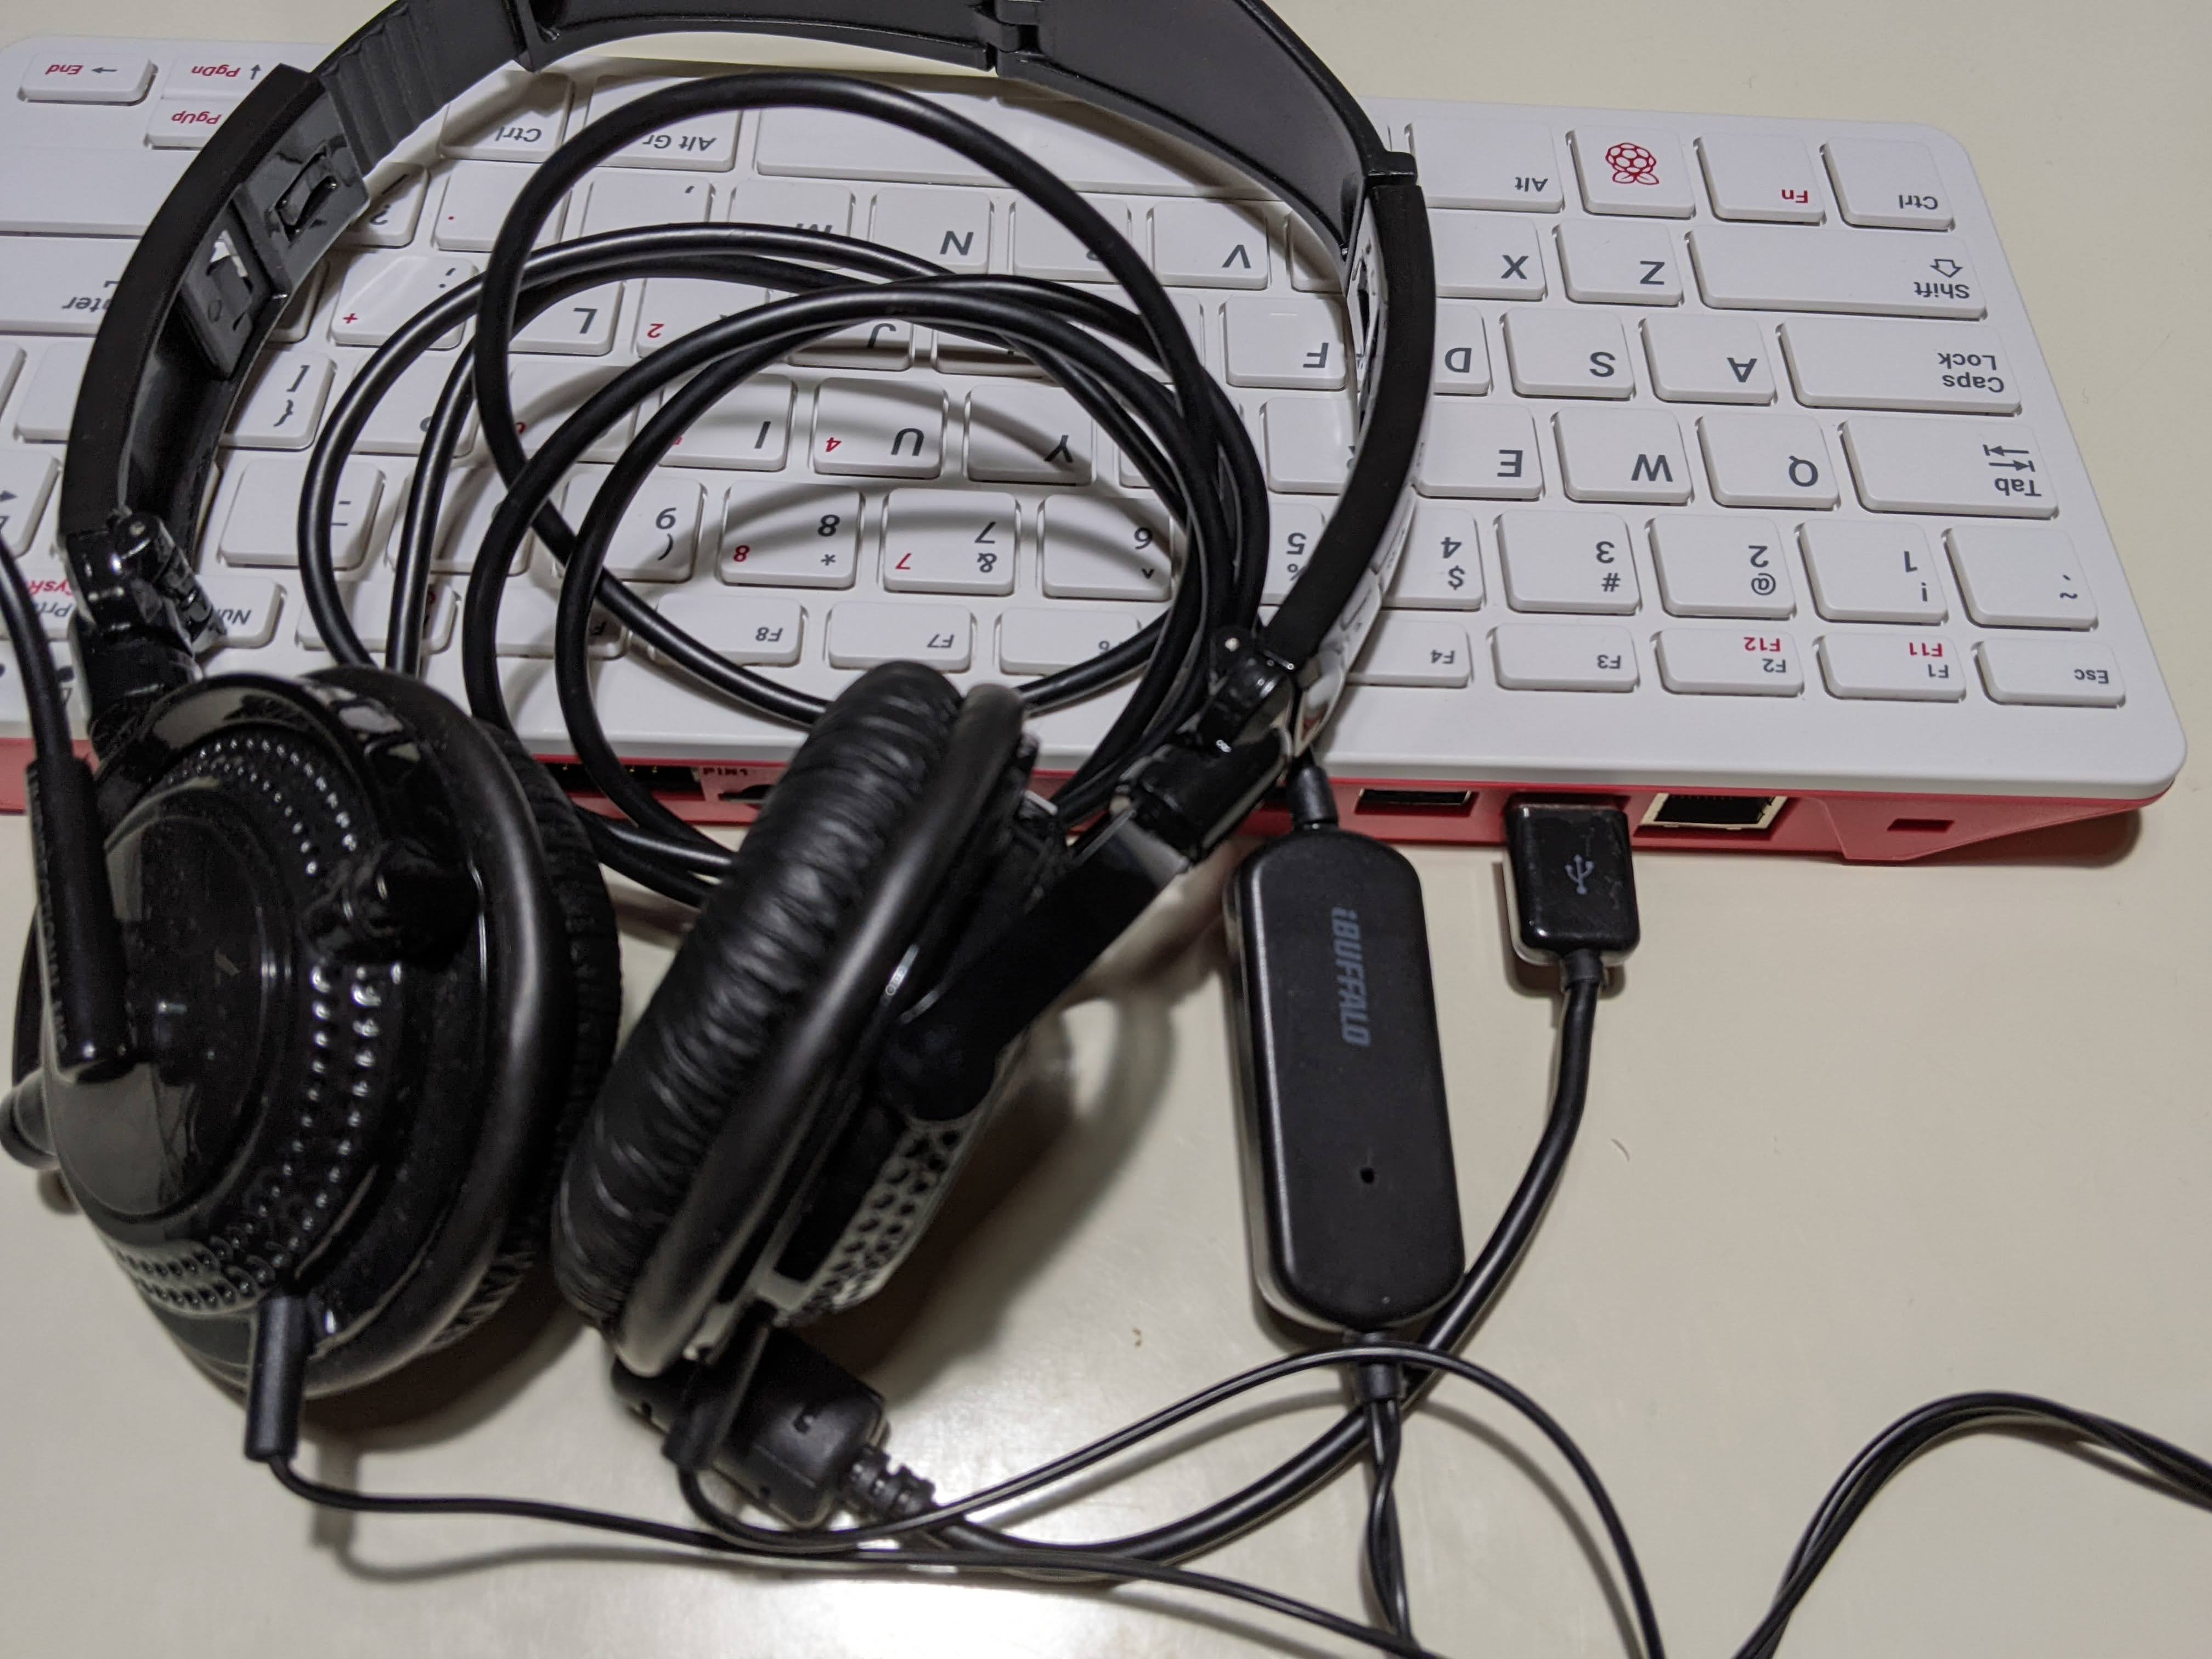
\includegraphics[width=.6\linewidth]{images/how_to_connect_headset.jpg}
    \caption{ヘッドセットのつなげかた}
    \label{つなげかた}
\end{center}
\end{figure}

ヘッドセットの出力音量はヘッドセットにつながっているコントローラーか、ディスプレイ右上のスピーカーのアイコンで調整できます。

\begin{figure}[H]
\begin{center}
    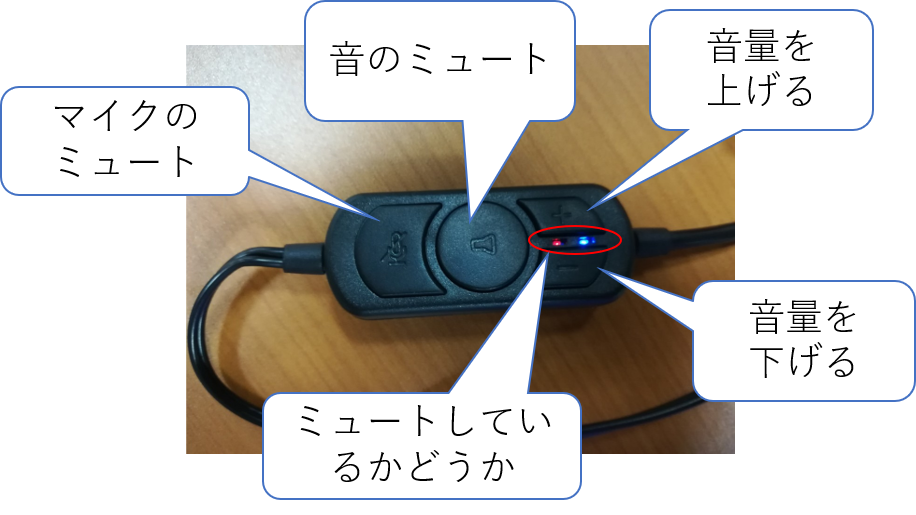
\includegraphics[width=.6\linewidth]{images/chap06/text06-img004.png}
    \caption{ヘッドセットのコントローラーの使い方}
    \label{ヘッドセットのコントローラーの使い方}
\end{center}
\end{figure}

ヘッドセットのコントローラーの一番左のボタンでマイクのミュートを切りかえることができます。ミュートとは音を消すことです。マイクがミュートしているときは赤色のLEDが光っています。マイクを使うときはミュートを\ruby{解除}{かい|じょ}して、赤色のLEDが光っていないようにしましょう。真ん中のボタンは音のミュートです。音が聞こえないときはここを\ruby{押}{お}してみましょう。右側のボタンは ``+" で音量を上げる、``-" で音量を下げることができます。
ヘッドセットの出力音量はディスプレイの右上にあるスピーカーのアイコンからも設定できます。

次に、音を出す音声デバイスを\ruby{選択}{せん|たく}しましょう。ディスプレイの右上にあるスピーカーアイコンを右クリックしてください。

\begin{minipage}[t]{0.48\linewidth}
    \begin{figure}[H]
        \begin{center}
            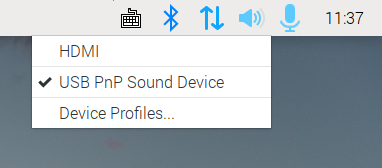
\includegraphics[width=\linewidth]{images/select_sink.png}
            \caption{使う音声デバイスの選択と設定}
            \label{使う音声デバイスの選択と設定}
        \end{center}
    \end{figure}
\end{minipage}
\begin{minipage}[t]{0.48\linewidth}
    \begin{figure}[H]
        \begin{center}
            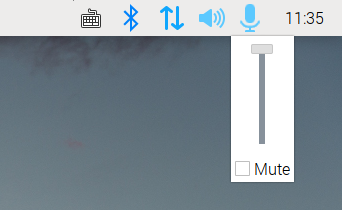
\includegraphics[width=\linewidth]{images/microphone_volume.png}
            \caption{マイクの入力音量の調節方法}
            \label{microphone_volume}
        \end{center}
    \end{figure}
\end{minipage}

図 \ref{使う音声デバイスの選択と設定} に使うことのできるデバイスが\ruby{表示}{ひょう|じ}されます。HDMIとはディスプレイのことです。これを左クリックするとディスプレイから音を出すことができます。\aruby{USB}{ユーエスビー} \aruby{PnP}{プラグ・アンド・プレイ} \aruby{Sound}{サウンド} \aruby{Device}{デバイス}は接続したヘッドセットのことです。ヘッドセットを使うときはこちらを左クリックします。
教室ではヘッドセットを使います。おうちでは、ディスプレイやテレビから音声を出力することもできます。

マイクの入力音量を変えるときはマイクのアイコンを左クリックし、表示されたスライドバーを調節します。



教室ではヘッドセットで音を聞き、ヘッドセットのマイクで音声を入力するので、図\ref{使う音声デバイスの選択と設定}のように USB PnP Sound Device を選択し、図\ref{microphone_volume}のようにマイクの入力音量を最大にしておきましょう。
